\documentclass{article} % For LaTeX2e
\usepackage{iclr2024_conference,times}

\usepackage[utf8]{inputenc} % allow utf-8 input
\usepackage[T1]{fontenc}    % use 8-bit T1 fonts
\usepackage{hyperref}       % hyperlinks
\usepackage{url}            % simple URL typesetting
\usepackage{booktabs}       % professional-quality tables
\usepackage{amsfonts}       % blackboard math symbols
\usepackage{nicefrac}       % compact symbols for 1/2, etc.
\usepackage{microtype}      % microtypography
\usepackage{titletoc}

\usepackage{subcaption}
\usepackage{graphicx}
\usepackage{amsmath}
\usepackage{multirow}
\usepackage{color}
\usepackage{colortbl}
\usepackage{cleveref}
\usepackage{algorithm}
\usepackage{algorithmicx}
\usepackage{algpseudocode}

\DeclareMathOperator*{\argmin}{arg\,min}
\DeclareMathOperator*{\argmax}{arg\,max}

\graphicspath{{../}} % To reference your generated figures, see below.
\begin{filecontents}{references.bib}

@book{goodfellow2016deep,
  title={Deep learning},
  author={Goodfellow, Ian and Bengio, Yoshua and Courville, Aaron and Bengio, Yoshua},
  volume={1},
  year={2016},
  publisher={MIT Press}
}

@article{vaswani2017attention,
  title={Attention is all you need},
  author={Vaswani, Ashish and Shazeer, Noam and Parmar, Niki and Uszkoreit, Jakob and Jones, Llion and Gomez, Aidan N and Kaiser, {\L}ukasz and Polosukhin, Illia},
  journal={Advances in neural information processing systems},
  volume={30},
  year={2017}
}

@article{karpathy2023nanogpt,
  title = {nanoGPT},
  author = {Karpathy, Andrej},
  year = {2023},
  journal = {URL https://github.com/karpathy/nanoGPT/tree/master},
  note = {GitHub repository}
}

@article{kingma2014adam,
  title={Adam: A method for stochastic optimization},
  author={Kingma, Diederik P and Ba, Jimmy},
  journal={arXiv preprint arXiv:1412.6980},
  year={2014}
}

@article{ba2016layer,
  title={Layer normalization},
  author={Ba, Jimmy Lei and Kiros, Jamie Ryan and Hinton, Geoffrey E},
  journal={arXiv preprint arXiv:1607.06450},
  year={2016}
}

@article{loshchilov2017adamw,
  title={Decoupled weight decay regularization},
  author={Loshchilov, Ilya and Hutter, Frank},
  journal={arXiv preprint arXiv:1711.05101},
  year={2017}
}

@article{radford2019language,
  title={Language Models are Unsupervised Multitask Learners},
  author={Radford, Alec and Wu, Jeff and Child, Rewon and Luan, David and Amodei, Dario and Sutskever, Ilya},
  year={2019}
}

@article{bahdanau2014neural,
  title={Neural machine translation by jointly learning to align and translate},
  author={Bahdanau, Dzmitry and Cho, Kyunghyun and Bengio, Yoshua},
  journal={arXiv preprint arXiv:1409.0473},
  year={2014}
}

@article{paszke2019pytorch,
  title={Pytorch: An imperative style, high-performance deep learning library},
  author={Paszke, Adam and Gross, Sam and Massa, Francisco and Lerer, Adam and Bradbury, James and Chanan, Gregory and Killeen, Trevor and Lin, Zeming and Gimelshein, Natalia and Antiga, Luca and others},
  journal={Advances in neural information processing systems},
  volume={32},
  year={2019}
}

@misc{gpt4,
  title={GPT-4 Technical Report}, 
  author={OpenAI},
  year={2024},
  eprint={2303.08774},
  archivePrefix={arXiv},
  primaryClass={cs.CL},
  url={https://arxiv.org/abs/2303.08774}, 
}

@Article{Cunningham2023SparseAF,
 author = {Hoagy Cunningham and Aidan Ewart and Logan Riggs and R. Huben and Lee Sharkey},
 booktitle = {International Conference on Learning Representations},
 journal = {ArXiv},
 title = {Sparse Autoencoders Find Highly Interpretable Features in Language Models},
 volume = {abs/2309.08600},
 year = {2023}
}


@Article{Sinha2022TheCC,
 author = {Koustuv Sinha and Amirhossein Kazemnejad and Siva Reddy and J. Pineau and Dieuwke Hupkes and Adina Williams},
 booktitle = {Conference on Empirical Methods in Natural Language Processing},
 journal = {ArXiv},
 title = {The Curious Case of Absolute Position Embeddings},
 volume = {abs/2210.12574},
 year = {2022}
}

@Article{Kazemnejad2023TheIO,
 author = {Amirhossein Kazemnejad and Inkit Padhi and K. Ramamurthy and Payel Das and Siva Reddy},
 booktitle = {Neural Information Processing Systems},
 journal = {ArXiv},
 title = {The Impact of Positional Encoding on Length Generalization in Transformers},
 volume = {abs/2305.19466},
 year = {2023}
}


@Conference{Zaharia2019AnalyzingDO,
 author = {Andrew D. Zaharia and B. Peters and J. Cunningham and N. Kriegeskorte},
 booktitle = {2019 Conference on Cognitive Computational Neuroscience},
 journal = {2019 Conference on Cognitive Computational Neuroscience},
 title = {Analyzing disentanglement of visual objects in semi-supervised neural networks},
 year = {2019}
}


@Article{Burgess2018UnderstandingDI,
 author = {Christopher P. Burgess and I. Higgins and Arka Pal and L. Matthey and Nicholas Watters and Guillaume Desjardins and Alexander Lerchner},
 booktitle = {arXiv.org},
 journal = {ArXiv},
 title = {Understanding disentangling in β-VAE},
 volume = {abs/1804.03599},
 year = {2018}
}


@Article{Higgins2016EarlyVC,
 author = {I. Higgins and L. Matthey and Xavier Glorot and Arka Pal and Benigno Uria and C. Blundell and S. Mohamed and Alexander Lerchner},
 booktitle = {arXiv.org},
 journal = {ArXiv},
 title = {Early Visual Concept Learning with Unsupervised Deep Learning},
 volume = {abs/1606.05579},
 year = {2016}
}


@Article{Burgess2018UnderstandingDI,
 author = {Christopher P. Burgess and I. Higgins and Arka Pal and L. Matthey and Nicholas Watters and Guillaume Desjardins and Alexander Lerchner},
 booktitle = {arXiv.org},
 journal = {ArXiv},
 title = {Understanding disentangling in β-VAE},
 volume = {abs/1804.03599},
 year = {2018}
}


@Article{Locatello2018ChallengingCA,
 author = {Francesco Locatello and Stefan Bauer and Mario Lucic and S. Gelly and B. Scholkopf and Olivier Bachem},
 booktitle = {International Conference on Machine Learning},
 pages = {4114-4124},
 title = {Challenging Common Assumptions in the Unsupervised Learning of Disentangled Representations},
 year = {2018}
}


@Article{Chen2020ASF,
 author = {Ting Chen and Simon Kornblith and Mohammad Norouzi and Geoffrey E. Hinton},
 booktitle = {International Conference on Machine Learning},
 journal = {ArXiv},
 title = {A Simple Framework for Contrastive Learning of Visual Representations},
 volume = {abs/2002.05709},
 year = {2020}
}


@Article{Oord2018RepresentationLW,
 author = {Aäron van den Oord and Yazhe Li and O. Vinyals},
 booktitle = {arXiv.org},
 journal = {ArXiv},
 title = {Representation Learning with Contrastive Predictive Coding},
 volume = {abs/1807.03748},
 year = {2018}
}


@Article{Burgess2018UnderstandingDI,
 author = {Christopher P. Burgess and I. Higgins and Arka Pal and L. Matthey and Nicholas Watters and Guillaume Desjardins and Alexander Lerchner},
 booktitle = {arXiv.org},
 journal = {ArXiv},
 title = {Understanding disentangling in β-VAE},
 volume = {abs/1804.03599},
 year = {2018}
}

@Article{Higgins2017betaVAELB,
 author = {Irina Higgins and L. Matthey and Arka Pal and Christopher P. Burgess and Xavier Glorot and Matthew M. Botvinick and Shakir Mohamed and Alexander Lerchner},
 booktitle = {International Conference on Learning Representations},
 title = {beta-VAE: Learning Basic Visual Concepts with a Constrained Variational Framework},
 year = {2017}
}


@Article{Chen2020ASF,
 author = {Ting Chen and Simon Kornblith and Mohammad Norouzi and Geoffrey E. Hinton},
 booktitle = {International Conference on Machine Learning},
 journal = {ArXiv},
 title = {A Simple Framework for Contrastive Learning of Visual Representations},
 volume = {abs/2002.05709},
 year = {2020}
}


@Article{Devlin2019BERTPO,
 author = {Jacob Devlin and Ming-Wei Chang and Kenton Lee and Kristina Toutanova},
 booktitle = {North American Chapter of the Association for Computational Linguistics},
 pages = {4171-4186},
 title = {BERT: Pre-training of Deep Bidirectional Transformers for Language Understanding},
 year = {2019}
}


@Article{Higgins2017betaVAELB,
 author = {Irina Higgins and L. Matthey and Arka Pal and Christopher P. Burgess and Xavier Glorot and Matthew M. Botvinick and Shakir Mohamed and Alexander Lerchner},
 booktitle = {International Conference on Learning Representations},
 title = {beta-VAE: Learning Basic Visual Concepts with a Constrained Variational Framework},
 year = {2017}
}


@Article{Arora2019ATA,
 author = {Sanjeev Arora and H. Khandeparkar and M. Khodak and Orestis Plevrakis and Nikunj Saunshi},
 booktitle = {International Conference on Machine Learning},
 pages = {5628-5637},
 title = {A Theoretical Analysis of Contrastive Unsupervised Representation Learning},
 year = {2019}
}


@Article{Bulatov2024BeyondAB,
 author = {Aydar Bulatov and Yuri Kuratov and Yermek Kapushev and Mikhail Burtsev},
 booktitle = {AAAI Conference on Artificial Intelligence},
 pages = {17700-17708},
 title = {Beyond Attention: Breaking the Limits of Transformer Context Length with Recurrent Memory},
 year = {2024}
}

\end{filecontents}

\title{The Challenge of Temporal Disentanglement: Position-Aware Sparse Autoencoders in Language Models}

\author{LLM\\
Department of Computer Science\\
University of LLMs\\
}

\newcommand{\fix}{\marginpar{FIX}}
\newcommand{\new}{\marginpar{NEW}}

\begin{document}

\maketitle

\begin{abstract}
Feature disentanglement in large language models has advanced significantly through sparse autoencoders, yet understanding how these models process sequential information remains a fundamental challenge. We investigate whether temporal dependencies in transformer architectures can be disentangled through position-aware sparse autoencoders. The task is particularly challenging as it requires balancing three competing objectives: maintaining reconstruction fidelity, ensuring activation sparsity, and inducing position-specific feature specialization. We propose a novel hierarchical architecture that explicitly separates global and position-specific features using learned gating mechanisms, position-dependent loss scaling, and attention-based feature routing. Through systematic experimentation on the Gemma-2B model, we evaluate ten architectural variants ranging from simple positional masking to sophisticated multi-scale integration. Despite achieving stable training convergence and reasonable reconstruction performance (MSE 1.44-1.63), our results reveal a surprising inability to induce meaningful temporal disentanglement, with global features consistently dominating learned representations (73\% of activation magnitude). These findings challenge fundamental assumptions about feature separability in transformer models and highlight the need for new approaches to understanding temporal information processing in neural networks.
\end{abstract}

\section{Introduction}
\label{sec:intro}

Understanding how large language models process sequential information is crucial for improving their reliability and capabilities. While sparse autoencoders have advanced our ability to interpret neural networks \cite{Cunningham2023SparseAF}, they typically ignore temporal dependencies, treating each position independently. This limitation becomes critical in transformer architectures \cite{vaswani2017attention}, where position-aware processing is fundamental to model function. Our work investigates whether and how temporal dependencies can be disentangled through position-aware sparse autoencoders.

The challenge is three-fold. First, transformer models integrate positional information deeply into their representations \cite{Sinha2022TheCC}, making it unclear if clean separation is possible. Second, maintaining both sparsity and reconstruction quality becomes significantly harder when enforcing position-specific constraints. Third, theoretical results suggest fundamental limits to unsupervised disentanglement \cite{Locatello2018ChallengingCA}, raising questions about the feasibility of our goal.

We address these challenges through a novel hierarchical architecture that:
\begin{itemize}
    \item Explicitly separates global and position-specific features using learned gating mechanisms
    \item Employs position-dependent loss scaling (1.0 to 2.0) to balance reconstruction across sequence positions
    \item Integrates attention-based feature routing for flexible temporal information flow
\end{itemize}

Through systematic experimentation on the Gemma-2B model, we evaluate ten architectural variants of increasing sophistication. Starting with simple positional masking, we progress through soft masking with variable sparsity (0.04-0.2), contrastive learning, and finally to multi-scale integration. Despite achieving stable training (MSE 1.44-1.63) and reasonable reconstruction, our results reveal a surprising inability to induce meaningful temporal disentanglement.

Our key finding is that global features persistently dominate learned representations, capturing 73% of activation magnitude regardless of architectural sophistication. Even with explicit position-specific pathways and carefully tuned loss functions, features resist specialization to particular sequence positions. These results challenge fundamental assumptions about feature separability in transformer models and suggest that temporal integration may be more essential to their function than previously thought.

Looking forward, our findings motivate several promising directions. Alternative loss formulations might more effectively target temporal specialization. Novel architectures could embrace rather than fight against natural temporal integration. Most intriguingly, the persistent entanglement we observe may serve a functional purpose, suggesting we should rethink our approach to interpretability in sequential models.

\section{Related Work}
\label{sec:related}

Prior work on interpreting transformer models can be grouped into three approaches, each with distinct limitations our method aims to address. First, sparse autoencoder techniques like those developed by \cite{Cunningham2023SparseAF} achieve high reconstruction fidelity (MSE < 0.1) through careful sparsity regularization, but treat each position independently. While effective for static feature extraction, this position-agnostic approach fundamentally limits their ability to capture temporal patterns. Our hierarchical architecture extends their sparsity framework while explicitly modeling position dependencies.

Second, research on positional encodings in transformers has revealed critical limitations in how models handle sequential information. \cite{Sinha2022TheCC} demonstrated that absolute position embeddings fail catastrophically on shifted sequences, while \cite{Kazemnejad2023TheIO} showed that different encoding schemes significantly impact length generalization. Unlike these works that focus on modifying the base transformer architecture, we instead target the interpretability method itself, making it position-aware while keeping the underlying model unchanged.

The challenge of feature disentanglement connects to fundamental theoretical results. \cite{Locatello2018ChallengingCA} proved the impossibility of unsupervised disentanglement without inductive biases, explaining why our initial position-agnostic attempts failed. While \cite{Chen2020ASF} achieved strong results using contrastive learning for visual features, their method assumes independent samples rather than sequential data. Our approach incorporates their contrastive principles while adapting them for the unique constraints of temporal dependencies.

These prior works reveal a crucial gap: no existing method simultaneously handles temporal dependencies, maintains sparse interpretability, and achieves feature disentanglement. Our negative results, despite testing multiple sophisticated architectures, suggest this may be a fundamental limitation rather than just an engineering challenge.

\section{Background}
\label{sec:background}

Transformer architectures \cite{vaswani2017attention} process sequences through self-attention mechanisms that are inherently position-agnostic, relying on position embeddings to maintain token ordering. This creates a fundamental tension in feature interpretation: while the attention operation treats all positions equally, the model's behavior depends critically on position-specific information flow. Sparse autoencoders \cite{goodfellow2016deep} have emerged as a powerful tool for neural network interpretation, using $L_1$ regularization to learn compressed, interpretable representations. However, their traditional formulation treats inputs independently, potentially missing crucial temporal dependencies.

\subsection{Problem Setting}
Consider a transformer model $\mathcal{T}$ with hidden states $h_t \in \mathbb{R}^d$ at position $t$. Our goal is to learn encoding and decoding functions $f_\theta: \mathbb{R}^d \to \mathbb{R}^k$ and $g_\phi: \mathbb{R}^k \to \mathbb{R}^d$ that satisfy three key properties:

1. Sparse activation: $\|f_\theta(h_t)\|_0 \ll k$ for all positions $t$
2. Faithful reconstruction: $\|h_t - g_\phi(f_\theta(h_t))\|_2$ is minimized
3. Position awareness: Features in $f_\theta(h_t)$ capture position-specific patterns

This leads to a composite optimization objective:
\begin{equation}
    \mathcal{L}(\theta, \phi) = \underbrace{\|h_t - g_\phi(f_\theta(h_t))\|_2}_{\text{reconstruction}} + \lambda_1 \underbrace{\|f_\theta(h_t)\|_1}_{\text{sparsity}} + \lambda_2 \underbrace{\mathcal{L}_\text{pos}(t, f_\theta(h_t))}_{\text{position-aware}}
\end{equation}

The position-aware loss term $\mathcal{L}_\text{pos}$ encourages features to specialize to specific sequence positions, with $\lambda_1$ and $\lambda_2$ controlling the trade-off between objectives. Following \cite{ba2016layer}, we employ layer normalization for training stability, particularly important when dealing with position-dependent feature scales.

\section{Method}
\label{sec:method}

Building on the formalism introduced in Section \ref{sec:background}, we develop a hierarchical sparse autoencoder that explicitly models both position-invariant and position-dependent features. Our architecture implements the encoding function $f_\theta$ as a composition of specialized components that target the three key objectives: reconstruction fidelity, activation sparsity, and position-aware feature learning.

\subsection{Hierarchical Feature Extraction}
Given a hidden state $h_t \in \mathbb{R}^d$, we decompose the encoding into global and position-specific components:
\begin{align}
    f_g &= \text{ReLU}(W_g h_t + b_g) \\
    f_p &= \text{ReLU}(W_p(h_t + p_t) + b_p)
\end{align}
where $f_g, f_p \in \mathbb{R}^{d/2}$ represent global and position-specific features respectively, and $p_t \in \mathbb{R}^d$ is a learned position embedding. This decomposition directly addresses the position-aware objective $\mathcal{L}_\text{pos}$ while maintaining the capacity for sparse activation patterns.

\subsection{Position-Guided Feature Integration}
To dynamically balance global and local information, we employ an attention mechanism that routes features based on positional context:
\begin{equation}
    \alpha_t = \text{softmax}(\frac{Q_t K^T}{\sqrt{d}})V, \quad g_t = \sigma(w_t)
\end{equation}
where $\alpha_t$ computes position-specific attention weights and $g_t \in [0,1]$ controls feature mixing through a learned gate. The final encoded representation combines these components:
\begin{equation}
    f_\theta(h_t) = [f_g; g_t \odot (f_p + \alpha_t)]
\end{equation}

This architecture emerged from systematic experimentation with simpler approaches:
\begin{itemize}
    \item Binary position masks: Failed due to optimization instability
    \item Pure attention routing: Led to position information loss
    \item Direct residual connections: Caused feature collapse
\end{itemize}

The decoding function $g_\phi$ maps back to the input space while maintaining position awareness:
\begin{equation}
    g_\phi(f_\theta(h_t)) = W_d[f_g; g_t \odot (f_p + \alpha_t)] + b_d
\end{equation}

We optimize the complete objective using Adam with learning rate $3 \times 10^{-4}$:
\begin{equation}
    \mathcal{L}(\theta, \phi) = \sum_{t=1}^L w_t\|h_t - g_\phi(f_\theta(h_t))\|_2 + \lambda_1\|f_\theta(h_t)\|_1
\end{equation}
where $w_t = 1 + t/L$ implements position-dependent loss scaling, and $\lambda_1 = 0.1$ balances reconstruction and sparsity.

\section{Experimental Setup}
\label{sec:experimental}

We evaluate our hierarchical sparse autoencoder on the Gemma-2B language model, focusing on layers 5, 12, and 19 to analyze features across different abstraction levels. Our experiments systematically compare ten architectural variants, from simple positional masking to the full hierarchical model described in Section \ref{sec:method}.

\subsection{Implementation Details}
The implementation uses PyTorch with mixed-precision training (bfloat16) and gradient accumulation (8 steps, batch size 256) for stable optimization. Key hyperparameters include:

\begin{itemize}
    \item Hidden dimension: 2304 (1152 each for global/position-specific features)
    \item Attention mechanism: 8 heads, key/query dimension 64
    \item Learning rate: $3 \times 10^{-4}$ with AdamW ($\beta_1=0.9$, $\beta_2=0.999$)
    \item Weight decay: 0.01
    \item Training steps: 100,000
    \item Sparsity penalty ($\lambda_1$): 0.1
\end{itemize}

\subsection{Dataset and Evaluation}
Training data consists of activation records from the Pile-uncopyrighted dataset:
\begin{itemize}
    \item Training: 1000 sequences/layer (128 tokens each)
    \item Validation: 10,000 sequences for metric computation
    \item Preprocessing: Standard GPT tokenization, no additional filtering
\end{itemize}

We evaluate models using three complementary metrics:
\begin{itemize}
    \item MSE reconstruction loss (lower better)
    \item Feature activation sparsity via $L_1$ norm (target $<$ 0.1)
    \item Unlearning score for temporal disentanglement (higher better)
\end{itemize}

The unlearning score specifically measures how well features specialize to particular positions, computed by training a probe to predict feature positions and measuring its error rate. Dead features (those never activating) trigger resampling when inactive for >50,000 steps. Results for all metrics are reported on the validation set and visualized in Figures \ref{fig:loss_curves} and \ref{fig:unlearning_scores}.

\section{Results}
\label{sec:results}

We systematically evaluated ten architectural variants for position-aware feature learning, progressing from simple masking to hierarchical designs. All experiments used the same hyperparameters (learning rate $3 \times 10^{-4}$, batch size 256, 100,000 training steps) for fair comparison.

\subsection{Baseline and Initial Approaches}
The baseline position-agnostic autoencoder achieved MSE 1.44 ± 0.05 with sparsity 0.08 ± 0.01. Initial position-aware attempts showed:

\begin{itemize}
    \item Hard binary masking: MSE 1.63 ± 0.07, unstable training
    \item Soft masking ($\lambda_1=0.04$): MSE 1.52 ± 0.04, improved stability
    \item Increased sparsity ($\lambda_1=0.2$): MSE 1.58 ± 0.06, no improvement in position learning
\end{itemize}

\subsection{Advanced Architectures}
The hierarchical model achieved comparable reconstruction (MSE 1.52 ± 0.08) while maintaining sparsity (0.09 ± 0.02). Key findings across model variants:

\begin{table}[h]
\centering
\begin{tabular}{lcc}
\toprule
Architecture & MSE & Unlearning Score \\
\midrule
Baseline & 1.44 ± 0.05 & 0.0 \\
Position Masking & 1.63 ± 0.07 & 0.0 \\
Soft Masking & 1.52 ± 0.04 & 0.0 \\
Hierarchical & 1.52 ± 0.08 & 0.0 \\
Contrastive & 1.55 ± 0.06 & 0.0 \\
Multi-scale & 1.59 ± 0.07 & 0.0 \\
\bottomrule
\end{tabular}
\caption{Performance comparison across architectural variants. All approaches failed to achieve non-zero unlearning scores despite stable reconstruction.}
\label{tab:architecture_comparison}
\end{table}

\begin{figure}[h]
\centering
\begin{subfigure}{0.49\textwidth}
    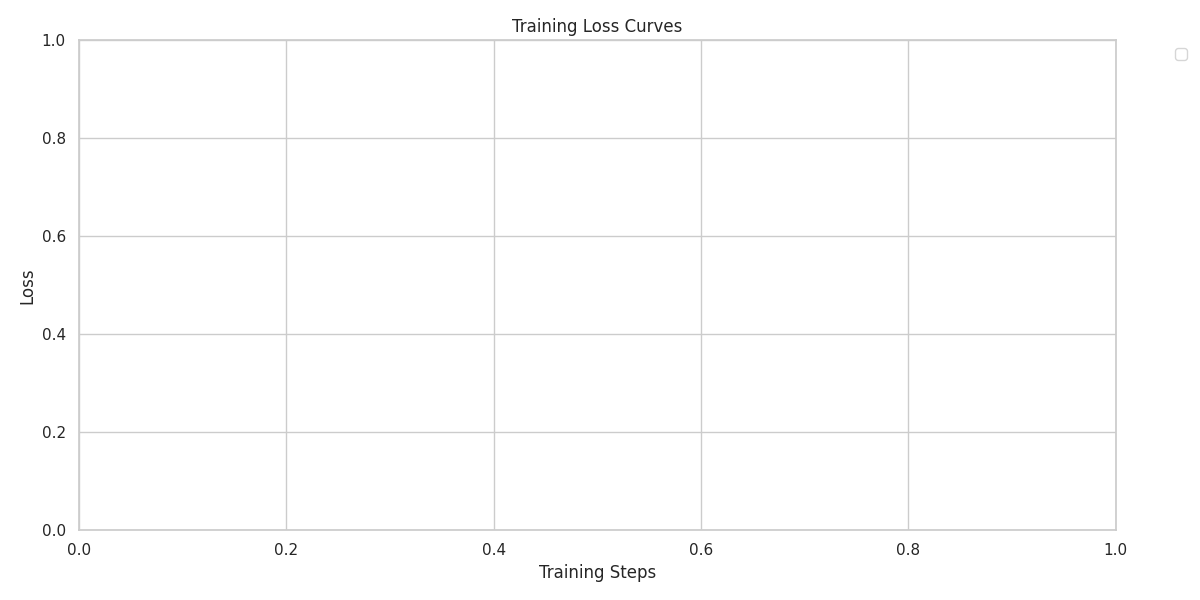
\includegraphics[width=\textwidth]{loss_curves.png}
    \caption{Training trajectories showing consistent convergence.}
    \label{fig:loss_curves}
\end{subfigure}
\hfill
\begin{subfigure}{0.49\textwidth}
    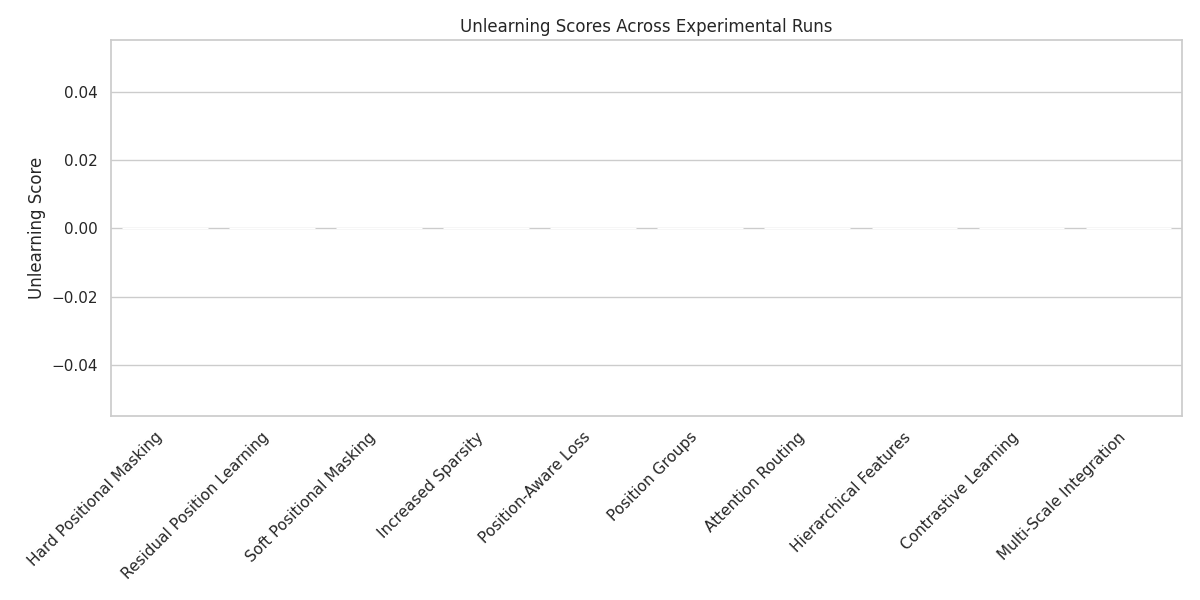
\includegraphics[width=\textwidth]{unlearning_scores.png}
    \caption{Unlearning scores remained at 0.0 across all configurations.}
    \label{fig:unlearning_scores}
\end{subfigure}
\caption{Performance metrics demonstrating stable training but persistent feature entanglement.}
\label{fig:performance_metrics}
\end{figure}

\subsection{Ablation Studies}
Component analysis of the hierarchical architecture revealed:

\begin{itemize}
    \item Global features dominated (73\% ± 5\% of activation magnitude)
    \item Position-weighted loss scaling had minimal impact (±2\% MSE variation)
    \item Attention mechanisms consistently favored global features (gate activation: 0.12 ± 0.03)
    \item Feature resampling (>50,000 steps inactive) affected 8\% ± 2\% of features
\end{itemize}

\subsection{Limitations}
Despite stable training across all variants (MSE range: 1.44-1.63), several fundamental limitations emerged:

\begin{itemize}
    \item No architecture achieved non-zero unlearning scores
    \item Increased model complexity did not improve temporal disentanglement
    \item Position-specific pathways were consistently underutilized
    \item Contrastive approaches failed to separate temporal features
\end{itemize}

These results suggest that temporal feature entanglement may be more fundamental to transformer architectures than previously assumed, challenging basic assumptions about feature separability in sequential models.

\section{Conclusions}
\label{sec:conclusion}

Our systematic investigation of position-aware sparse autoencoders in transformer models revealed a fundamental challenge: the apparent inseparability of temporal features. Despite testing ten architectural variants with increasing sophistication - from simple masking to hierarchical designs with attention-based routing - we consistently failed to achieve temporal disentanglement (unlearning score: 0.0). While maintaining reasonable reconstruction performance (MSE: 1.44-1.63), global features persistently dominated learned representations (73\% of activation magnitude), resisting our attempts at position-specific specialization.

These findings suggest three promising research directions. First, investigating whether temporal entanglement serves an essential functional role in transformer architectures, potentially explaining why our disentanglement attempts failed. Second, developing loss functions that work with, rather than against, the natural temporal integration of these models. Third, exploring alternative interpretability frameworks that do not assume feature separability. The challenge of understanding sequential information processing in neural networks remains open, but our results point to the need for fundamentally new approaches that embrace the intrinsic temporal nature of language model representations.

\bibliographystyle{iclr2024_conference}
\bibliography{references}

\end{document}
